\documentclass[border=4pt]{standalone}
\usepackage[T1]{fontenc}
\usepackage{lmodern}
\usepackage{amsmath}
\usepackage{tikz}
\usetikzlibrary{positioning,arrows.meta,fit,backgrounds,calc}
\begin{document}
\sffamily\footnotesize
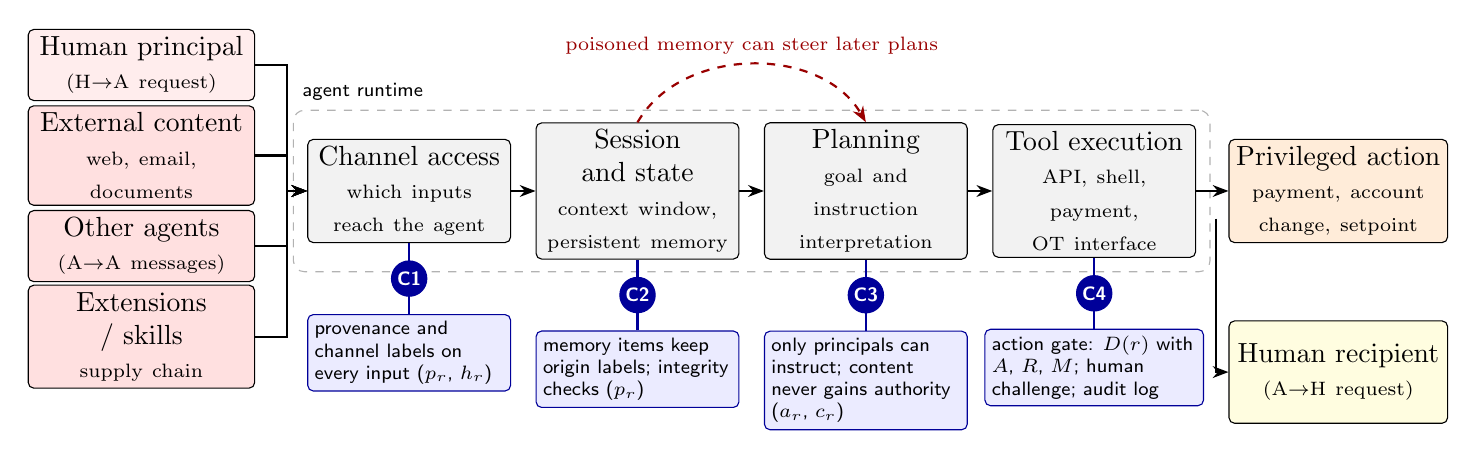
\begin{tikzpicture}[
  box/.style={draw, rounded corners=2pt, align=center, text width=24mm, minimum height=13mm, inner sep=2.5pt},
  src/.style={box, fill=red!7, text width=27mm, minimum height=9mm},
  st/.style={box, fill=gray!10},
  cz/.style={draw=blue!60!black, fill=blue!8, rounded corners=2pt, align=flush left, text width=24mm, inner sep=2.5pt, font=\sffamily\scriptsize},
  cc/.style={circle, draw=blue!60!black, fill=blue!60!black, text=white, inner sep=1pt, font=\sffamily\scriptsize\bfseries},
  arr/.style={-{Stealth[length=2mm]}, thick},
  bad/.style={-{Stealth[length=2mm]}, thick, red!60!black, dashed}
]
% untrusted sources
\node[src] (s1) at (0, 1.6) {Human principal\\{\scriptsize (H$\rightarrow$A request)}};
\node[src, fill=red!12] (s2) at (0, 0.45) {External content\\{\scriptsize web, email, documents}};
\node[src, fill=red!12] (s3) at (0,-0.7) {Other agents\\{\scriptsize (A$\rightarrow$A messages)}};
\node[src, fill=red!12] (s4) at (0,-1.85) {Extensions / skills\\{\scriptsize supply chain}};
% agent lifecycle stages (trust boundaries after Ma et al.)
\node[st] (b1) at (3.4,0) {Channel access\\{\scriptsize which inputs reach the agent}};
\node[st] (b2) at (6.3,0) {Session and state\\{\scriptsize context window, persistent memory}};
\node[st] (b3) at (9.2,0) {Planning\\{\scriptsize goal and instruction interpretation}};
\node[st] (b4) at (12.1,0) {Tool execution\\{\scriptsize API, shell, payment, OT interface}};
\node[box, fill=orange!15, text width=26mm] (act) at (15.2,0) {Privileged action\\{\scriptsize payment, account change, setpoint}};
\node[box, fill=yellow!12, text width=26mm] (hum) at (15.2,-2.3) {Human recipient\\{\scriptsize (A$\rightarrow$H request)}};
\begin{scope}[on background layer]
\node[draw=gray!60, dashed, rounded corners, fit=(b1)(b4), inner sep=5pt, label={[font=\sffamily\scriptsize, anchor=south west]north west:agent runtime}] (rt) {};
\end{scope}
\foreach \s in {s1,s2,s3,s4} \draw[arr] (\s.east) -- ++(4mm,0) |- (b1.west);
\draw[arr] (b1) -- (b2); \draw[arr] (b2) -- (b3); \draw[arr] (b3) -- (b4); \draw[arr] (b4) -- (act);
\draw[arr] ($(b4.east)+(0.25,-0.35)$) |- (hum.west);
\draw[bad] (b2.north) to[out=60, in=120] node[above, font=\scriptsize, text=red!60!black]{poisoned memory can steer later plans} (b3.north);
% CZT checkpoints
\node[cz, below=9mm of b1] (c1) {provenance and channel labels on every input ($p_r$, $h_r$)};
\node[cz, below=9mm of b2] (c2) {memory items keep origin labels; integrity checks ($p_r$)};
\node[cz, below=9mm of b3] (c3) {only principals can instruct; content never gains authority ($a_r$, $c_r$)};
\node[cz, below=9mm of b4, text width=26mm] (c4) {action gate: $D(r)$ with $A$, $R$, $M$; human challenge; audit log};
\foreach \i/\b in {1/b1,2/b2,3/b3,4/b4} {\draw[thick, blue!60!black] (c\i.north) -- (\b.south); \node[cc] at ($(\b.south)!0.5!(c\i.north)$) {C\i};}
\end{tikzpicture}
\end{document}
